%%%%%%%%%%%%%%%%%%%%%%%%%%%%%%%%%%%%%%%%%
% Beamer Presentation
% LaTeX Template
% Version 2.0 (March 8, 2022)
%
% This template originates from:
% https://www.LaTeXTemplates.com
%
% Author:
% Vel (vel@latextemplates.com)
%
% License:
% CC BY-NC-SA 4.0 (https://creativecommons.org/licenses/by-nc-sa/4.0/)
%
%%%%%%%%%%%%%%%%%%%%%%%%%%%%%%%%%%%%%%%%%

%----------------------------------------------------------------------------------------
%	PACKAGES AND OTHER DOCUMENT CONFIGURATIONS
%----------------------------------------------------------------------------------------
\documentclass[
  24pt, % Set the default font size, options include: 8pt, 9pt, 10pt, 11pt, 12pt, 14pt, 17pt, 20pt
  %t, % Uncomment to vertically align all slide content to the top of the slide, rather than the default centered
  aspectratio=169, % Uncomment to set the aspect ratio to a 16:9 ratio which matches the aspect ratio of 1080p and 4K screens and projectors
]{beamer}

\graphicspath{{Images/}{./}} % Specifies where to look for included images (trailing slash required)

\usepackage{booktabs} % Allows the use of \toprule, \midrule and \bottomrule for better rules in tables

%----------------------------------------------------------------------------------------
%	SELECT LAYOUT THEME
%----------------------------------------------------------------------------------------

% Beamer comes with a number of default layout themes which change the colors and layouts of slides. Below is a list of all themes available, uncomment each in turn to see what they look like.

%\usetheme{default}
%\usetheme{AnnArbor}
%\usetheme{Antibes}
%\usetheme{Bergen}
%\usetheme{Berkeley}
%\usetheme{Berlin}
\usetheme{Boadilla} %me gusta
%\usetheme{CambridgeUS}
%\usetheme{Copenhagen}
%\usetheme{Darmstadt}
%\usetheme{Dresden}
%\usetheme{Frankfurt}
%\usetheme{Goettingen} %dos dos
%\usetheme{Hannover} %dos dos
%\usetheme{Ilmenau}
%\usetheme{JuanLesPins}
%\usetheme{Luebeck}
%\usetheme{Madrid}
%\usetheme{Malmoe}
%\usetheme{Marburg}
%\usetheme{Montpellier}
%\usetheme{PaloAlto}
%\usetheme{Pittsburgh}
%\usetheme{Rochester} %muy flat
%\usetheme{Singapore}
%\usetheme{Szeged}
%\usetheme{Warsaw}

%----------------------------------------------------------------------------------------
%	SELECT COLOR THEME
%----------------------------------------------------------------------------------------

% Beamer comes with a number of color themes that can be applied to any layout theme to change its colors. Uncomment each of these in turn to see how they change the colors of your selected layout theme.

%\usecolortheme{albatross}
%\usecolortheme{beaver}
%\usecolortheme{beetle}
%\usecolortheme{crane}
%\usecolortheme{dolphin}
%\usecolortheme{dove}
%\usecolortheme{fly}
%\usecolortheme{lily} %default
%\usecolortheme{monarca}
%\usecolortheme{seagull}
%\usecolortheme{seahorse}
%\usecolortheme{spruce}
%\usecolortheme{whale}
%\usecolortheme{wolverine}

%----------------------------------------------------------------------------------------
%	SELECT FONT THEME & FONTS
%----------------------------------------------------------------------------------------

% Beamer comes with several font themes to easily change the fonts used in various parts of the presentation. Review the comments beside each one to decide if you would like to use it. Note that additional options can be specified for several of these font themes, consult the beamer documentation for more information.

\usefonttheme{default} % Typeset using the default sans serif font
%\usefonttheme{serif} % Typeset using the default serif font (make sure a sans font isn't being set as the default font if you use this option!)
%\usefonttheme{structurebold} % Typeset important structure text (titles, headlines, footlines, sidebar, etc) in bold
%\usefonttheme{structureitalicserif} % Typeset important structure text (titles, headlines, footlines, sidebar, etc) in italic serif
%\usefonttheme{structuresmallcapsserif} % Typeset important structure text (titles, headlines, footlines, sidebar, etc) in small caps serif

%------------------------------------------------

%\usepackage{mathptmx} % Use the Times font for serif text
\usepackage{palatino} % Use the Palatino font for serif text

\usepackage[ruled,vlined]{algorithm2e}
%\usepackage{helvet} % Use the Helvetica font for sans serif text
\usepackage[default]{opensans} % Use the Open Sans font for sans serif text
\usepackage[spanish]{babel}
\usepackage{dirtree}
\usepackage{xcolor}
%\usepackage[default]{FiraSans} % Use the Fira Sans font for sans serif text
%\usepackage[default]{lato} % Use the Lato font for sans serif text

\usepackage[scaled]{helvet}
\usepackage[round]{natbib}
%\newcommand{\newblock}{}

\usepackage{rotating}

\newcommand\FourQuad[4]{%
  \begin{minipage}[b][.33\textheight][t] 
    {.48\textwidth}#1\end{minipage}\hfill%
    \begin{minipage}[b][.33\textheight][t] 
      {.48\textwidth}#2\end{minipage}\\[0.5em]
      \begin{minipage}[b][.33\textheight][t] 
        {.48\textwidth}#3\end{minipage}\hfill
        \begin{minipage}[b][.33\textheight][t] 
          {.48\textwidth}#4\end{minipage}%
}

\usepackage{tikz}
%\usetikzlibrary{arrows,shapes,positioning,shadows,trees,quotes}


%\tikzset{
%  basic/.style  = {draw, text width=2cm, drop shadow, font=\sffamily, rectangle},
%  root/.style   = {basic, rounded corners=2pt, thin, align=center,
%                   fill=green!30},
%  level 2/.style = {basic, rounded corners=6pt, thin,align=center, fill=green!60,
%                   text width=8em},
%  level 3/.style = {basic, thin, align=left, fill=pink!60, text width=6.5em}
%}

\usetikzlibrary{calc}

\tikzstyle{part} = [rectangle, rounded corners, minimum width=3cm, minimum height=1cm,     align=center, draw=black]
\tikzstyle{chapter} = [rectangle, rounded corners, minimum width=3cm, minimum height=1cm,     align=center, draw=black, text width=3.5cm]
\tikzstyle{arrow} = [thick, ->]

\usepackage{array} % needed for \arraybackslash
\usepackage{graphicx}
\usepackage{adjustbox} % for \adjincludegraphics

\usepackage{subcaption}
\usepackage{bibentry}
%\bibliographystyle{apalike}
\usepackage{chngcntr}
\usepackage{lipsum}% http://ctan.org/pkg/lipsum
\usepackage{hanging}% http://ctan.org/pkg/hanging

\usepackage{xcolor,colortbl}
\usepackage{multirow}

\usepackage{animate}
\usepackage{multicol}
\usepackage{tabularx,booktabs}
\usepackage{forloop}
\usepackage{ragged2e}

\usepackage{bbding} %palomitas checkmark
\usepackage{pifont}
\usepackage{lipsum,tabularx}

\newcounter{loopcntr}

%----------------------------------------------------------------------------------------
%	SELECT INNER THEME
%----------------------------------------------------------------------------------------

% Inner themes change the styling of internal slide elements, for example: bullet points, blocks, bibliography entries, title pages, theorems, etc. Uncomment each theme in turn to see what changes it makes to your presentation.

\useinnertheme{circles}

%----------------------------------------------------------------------------------------
%	SELECT OUTER THEME
%----------------------------------------------------------------------------------------

% Outer themes change the overall layout of slides, such as: header and footer lines, sidebars and slide titles. Uncomment each theme in turn to see what changes it makes to your presentation.

\setbeamertemplate{footline}[frame number] % Uncomment this line to replace the footer line in all slides with a simple slide count
\setbeamertemplate{navigation symbols}{} % Uncomment this line to remove the navigation symbols from the bottom of all slides

%----------------------------------------------------------------------------------------
%	PRESENTATION INFORMATION
%----------------------------------------------------------------------------------------

\title[PRESENTACION 3]{%\centering\includegraphics[width=10cm]{swarm_drones}\\
  Definición de requerimientos}

%\subtitle{Optional Subtitle} % Presentation subtitle, remove this command if a subtitle isn't required

\author[]{Luis Alberto Ballado Aradias\\[\baselineskip]}

\institute[CINVESTAV]{
  CINVESTAV UNIDAD TAMAULIPAS \\
}


\date[\today]{Cd. Victoria, Tamaulipas - 28 Enero 2025} % Presentation date or conference/meeting name, the optional parameter can contain a shortened version to appear on the bottom of every slide, while the required parameter value is output to the title slide

%\titlegraphic{\hspace*{8.75cm}~%
%   \includegraphics[width=0.8cm]{cinvestavlogo}
%}

%----------------------------------------------------------------------------------------

\counterwithin*{footnote}{page}
\newcommand\footcite[1]{\footnote{\bibentry{#1}}\label{\thepage:#1}}
\newcommand\secondcite[1]{\textsuperscript{\ref{\thepage:#1}}}

\newcommand{\rpt}[2][1]{%
  \forloop{loopcntr}{0}{\value{loopcntr}<#1}{#2}%
}
\newcommand{\on}[1][1]{
  \forloop{loopcntr}{0}{\value{loopcntr}<#1}{&\cellcolor{gray}}
}
\newcommand{\onok}[1][1]{
  \forloop{loopcntr}{0}{\value{loopcntr}<#1}{&\cellcolor{green}}
}
\newcommand{\off}[1][1]{
  \forloop{loopcntr}{0}{\value{loopcntr}<#1}{&\cellcolor{white}}
}

\addtolength{\textheight}{90pt}

\newcommand{\I}{\mathbb{I}}
\newcommand{\K}{\mathbb{K}}
\newcommand{\N}{\mathbb{N}}
\newcommand{\Q}{\mathbb{Q}}
\newcommand{\R}{\mathbb{R}}
\newcommand{\Z}{\mathbb{Z}}

\newcommand{\specialcell}[2][c]{%
  \begin{tabular}[#1]{@{}c@{}}#2\end{tabular}}


\begin{document}

%----------------------------------------------------------------------------------------
%	TITLE SLIDE
%----------------------------------------------------------------------------------------

\begin{frame}
  \titlepage % Output the title slide, automatically created using the text entered in the PRESENTATION INFORMATION block above
\end{frame}

%----------------------------------------------------------------------------------------
%	TABLE OF CONTENTS SLIDE
%----------------------------------------------------------------------------------------

% The table of contents outputs the sections and subsections that appear in your presentation, specified with the standard \section and \subsection commands. You may either display all sections and subsections on one slide with \tableofcontents, or display each section at a time on subsequent slides with \tableofcontents[pausesections]. The latter is useful if you want to step through each section and mention what you will discuss.
\AtBeginSection[]
{
  \begin{frame}
    \frametitle{Contenido} % Slide title, remove this command for no title
    \tableofcontents[currentsection] % Output the table of contents (all sections on one slide)
    %\tableofcontents[pausesections] % Output the table of contents (break sections up across separate slides)
  \end{frame}
}

\pretocmd{\tableofcontents}{\thispagestyle{empty}}{}{}

%----------------------------------------------------------------------------------------
%	PRESENTATION BODY SLIDES
%----------------------------------------------------------------------------------------

% Sección 1: Introducción
\section{Introducción}
\begin{frame}{Ingenieria de Software}

  \begin{center}
    \begin{minipage}{0.38\linewidth}
      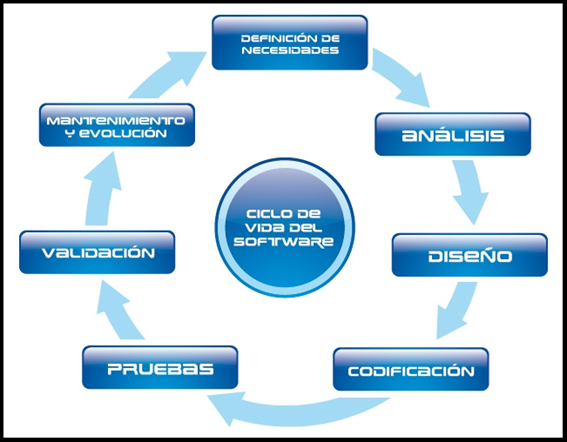
\includegraphics[width=\linewidth]{ciclo_vida_software.png}
      \captionof{figure}{clásico}
    \end{minipage}%
    \hfill
    \begin{minipage}{0.49\linewidth}
      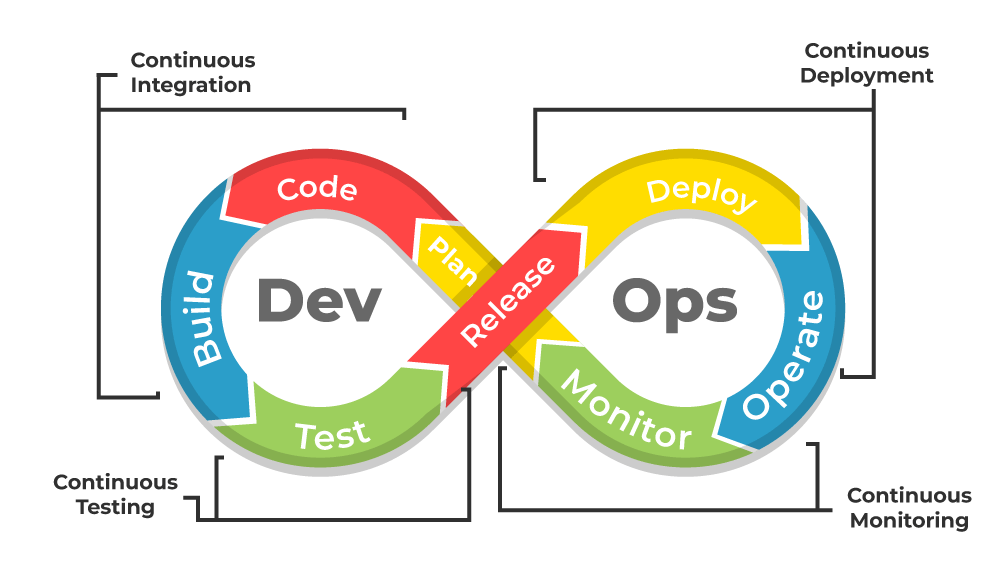
\includegraphics[width=\linewidth]{DevOps.png}
      \captionof{figure}{moderno}
    \end{minipage}
    \captionof{figure}{Ciclo de vida del software}
  \end{center}
\end{frame}  

\begin{frame}{¿Qué es un requerimiento?}
  Un requerimiento es:
  \begin{enumerate}
  \item .. lo que un sistema debe hacer
  \item .. limitaciones y restricciones conocidas
  \item .. nivel de rendimiento o calidad que se espera del sistema
  \end{enumerate}
  \vspace{0.5cm}
  \pause
  
  La primera definición es para \textbf{requerimientos funcionales.}\\
  La segunda y tercera son \textbf{requerimientos no funcionales.}
  
\end{frame}

\begin{frame}{Toma de requerimientos}
  \begin{itemize}
  \item Entrevistas (Lenguaje natural)
  \item Modelado de requerimientos
    \begin{itemize}
    \item grafos - UML
    \item formulas - representaciones matemáticas
    \item código - pseudocode / prototipos
    \end{itemize}
  \end{itemize}
  \vspace{0.5cm}
  \pause
  Limitantes
  \begin{itemize}
  \item Objetivos de la tarea a realizar
  \item Stakeholders (Interesados)
  \item Restricciones de la tarea a realizar
  \end{itemize}
\end{frame}

\begin{frame}{Problemas en toma de requerimientos}
  \begin{itemize}
  \item Incompletos / Ocultos 
  \item Inconsistentes
  \item Terminologia
  \item Responsabilidades no claras
  \item Comunicación
  \item Cambio de objetivos
  \item Requerimientos inviables
  \item Los interesados desconocen ciertos procesos
  \item Requerimientos no especificados
  \end{itemize}
\end{frame}

\section{IEEE 29148-2011}
\begin{frame}{Introducción a IEEE 29148-2011}
\framesubtitle{¿Qué es IEEE 29148-2011?}
\begin{itemize}
    \item Una norma para la ingeniería de requisitos en sistemas y software.
    \item Proporciona directrices para los procesos y actividades relacionados con la ingeniería de requisitos a lo largo del ciclo de vida del sistema o software.
\end{itemize}
\vspace{0.5cm}
Propósito
\begin{itemize}
    \item Asegurar que los requisitos estén bien definidos, sean medibles y trazables.
    \item Mejorar la comunicación entre los interesados.
    \item Apoyar el desarrollo de sistemas y software de alta calidad.
\end{itemize}
\end{frame}

% Sección 2: Conceptos Clave

%\begin{frame}{Conceptos Clave en IEEE 29148-2011}
%\framesubtitle{Tipos de Requisitos}
%\begin{itemize}
%    \item \textbf{Requisitos Funcionales:} Lo que el sistema debe hacer.
%    \item \textbf{Requisitos No Funcionales:} Restricciones y atributos de calidad (por ejemplo, rendimiento, seguridad).
%    \item \textbf{Requisitos del Usuario:} Necesidades de los usuarios finales.
%    \item \textbf{Requisitos del Sistema:} Requisitos de alto nivel para todo el sistema.
%\end{itemize}
%\vspace{0.5cm}
%Trazabilidad
%\begin{itemize}
%    \item Asegura que los requisitos estén vinculados a sus fuentes y a los artefactos de diseño, implementación y pruebas.
%\end{itemize}
%\end{frame}

% Sección 3: Estructura de la Norma
%\begin{frame}{Estructura de la Norma}
%\framesubtitle{Secciones de IEEE 29148-2011}
%\begin{itemize}
%    \item \textbf{Alcance:} Define el propósito y la aplicabilidad de la norma.
%    \item \textbf{Referencias Normativas:} Lista de normas relacionadas.
%    \item \textbf{Términos y Definiciones:} Terminología clave utilizada en la norma.
%    \item \textbf{Proceso de Ingeniería de Requisitos:} Modelo detallado del proceso de IR.
%    \item \textbf{Documentación de Requisitos:} Directrices para crear documentos de requisitos.
%    \item \textbf{Anexos:} Información adicional, incluyendo plantillas y ejemplos.
%\end{itemize}
%\end{frame}

% Sección 4: Cómo Usar la Norma
\begin{frame}{Cómo Usar IEEE 29148-2011}
\framesubtitle{Pasos para Aplicar la Norma}
\begin{itemize}
    \item \textbf{Elicitación:} Recopilar requisitos de los interesados.
    \item \textbf{Análisis:} Analizar requisitos para verificar su viabilidad, consistencia y completitud.
    \item \textbf{Especificación:} Documentar los requisitos de manera clara y sin ambigüedades.
    \item \textbf{Validación:} Verificar que los requisitos satisfacen las necesidades de los interesados.
    \item \textbf{Gestión:} Rastrear cambios y mantener la trazabilidad.
\end{itemize}
La norma incluye plantillas para documentos de requisitos, como la Especificación de Requisitos de Software (SRS).\
\end{frame}

\begin{frame}{Plantillas}
  \begin{itemize}
  \item Que plantillas 
  \item ..
  \item ..
  \end{itemize}
\end{frame}

% Sección 5: Cuándo Usar la Norma
\begin{frame}{Cuándo Usar IEEE 29148-2011}
\begin{itemize}
    \item \textbf{Proyectos de Desarrollo de Software:} Especialmente sistemas grandes, complejos o de seguridad crítica.
    \item \textbf{Ingeniería de Sistemas:} Para sistemas que incluyen componentes de hardware y software.
    \item \textbf{Industrias Reguladas:} Como aeroespacial, automotriz, salud y defensa, donde el cumplimiento de normas es obligatorio.
\end{itemize}
\vspace{0.5cm}
Cuándo Aplicar
\begin{itemize}
    \item Durante las fases iniciales de un proyecto para definir requisitos.
    \item A lo largo del ciclo de vida del proyecto para gestionar cambios y asegurar la trazabilidad.
    \item Durante auditorías o evaluaciones para demostrar el cumplimiento de normas industriales.
\end{itemize}
\end{frame}

% Sección 6: Beneficios
\begin{frame}{Beneficios y consideraciones}
Beneficios
\begin{itemize}
\item Asegura que los requisitos sean completos, consistentes y verificables.
\item Proporciona un lenguaje y marco común para los interesados.
\item Ayuda a identificar y mitigar riesgos temprano en el proyecto.
\item Facilita la adherencia a normas regulatorias e industriales.
\end{itemize}
Consideraciones
\begin{itemize}
\item Asegurar que todos los miembros del equipo estén capacitados en las prácticas de la norma.
\item Requiere tiempo y esfuerzo para adoptarla y mantenerla.
\end{itemize}
\end{frame}

\section{The Easy Approach to Requirements Syntax: EARS}

\begin{frame}{The Easy Approach to Requirements Syntax: EARS}
  Método útil y popular que ha sido adoptado por muchas organizaciones en el campo de la ingeniería de requisitos. Esto se debe a sus patrones de sintaxis fáciles de aprender y aplicar. EARS es un método simple y lógico para construir requisitos en lenguaje natural claros.
\end{frame}

\begin{frame}{Patrones EARS}
  
\end{frame}

\begin{frame}{Ejemplos:}
  \begin{itemize}
  \item Ubicuidad: el software debe estar escrito en Python.
  \item Impulsado por eventos: cuando se recibe el dinero, la aplicación debe enviar una notificación.
  \item Comportamiento no deseado: si la contraseña se ingresa incorrectamente, la aplicación mostrará un mensaje de error.
  \item Impulsado por estado: cuando se está en modo No molestar, el software silenciará las llamadas entrantes.
  \item Opcional: cuando el puerto DP está presente, el software debe permitir al usuario mostrar la frecuencia de actualización máxima admitida.
  \item Complejo: cuando se presiona el botón de marcha atrás una vez, si el software detecta que la marcha atrás no está en su lugar, el software mostrará una notificación emergente.
  \end{itemize}
\end{frame}

\begin{frame}{¿Cuándo no usar EARS?}
  \begin{enumerate}
  \item Cuando el requerimiento se extiende de complejidad
  \item Si se tienen más de tres precondiciones
  \item Cuando los requerimientos son matemáticos
  \end{enumerate}
\end{frame}

% Sección 9: Conclusión
\begin{frame}{Conclusión}
\framesubtitle{Resumen}
\begin{itemize}
    \item IEEE 29148-2011 es una norma integral para la ingeniería de requisitos que ayuda a garantizar sistemas y software de alta calidad.
    \item Proporciona un enfoque estructurado para definir, documentar y gestionar requisitos.
\end{itemize}

\framesubtitle{Reflexiones Finales}
\begin{itemize}
    \item Adoptar IEEE 29148-2011 puede llevar a proyectos más exitosos, especialmente en entornos complejos o regulados.
    \item Considerar la norma como una herramienta valiosa en tu kit de ingeniería de sistemas y software.
\end{itemize}
\end{frame}


\begin{frame}[allowframebreaks,noframenumbering]{Bibliografía}
  \tiny
  \bibliographystyle{abbrvnat}
  \bibliography{test}
\end{frame}

\end{document} 
